
%(BEGIN_QUESTION)
% Copyright 2016, Tony R. Kuphaldt, released under the Creative Commons Attribution License (v 1.0)
% This means you may do almost anything with this work of mine, so long as you give me proper credit

Explain how the following systems (analog electronic versus pneumatic) are similar in their behavior:

$$\includegraphics[width=15.5cm]{i03928x01.eps}$$

\vskip 10pt

Explain how the following systems (analog electronic versus pneumatic) are similar in their behavior:

$$\includegraphics[width=15.5cm]{i03928x02.eps}$$

\vskip 20pt \vbox{\hrule \hbox{\strut \vrule{} {\bf Further exploration . . . (optional)} \vrule} \hrule}

Research the work of Harold Black in his patent (``Wave Translation System,'' U.S. Patent number 2,102,671 filed in 1932 and granted in 1937), when he applied the principle of {\it negative feedback} to the design of telephone amplifier circuits.  How well was this novel concept accepted by the professional community?


\vskip 20pt \vbox{\hrule \hbox{\strut \vrule{} {\bf Suggestions for Socratic discussion} \vrule} \hrule}

\begin{itemize}
\item{} Feedback systems are highly non-intuitive, and therefore cause much grief for students learning to master them.  Discuss how to use ``thought experiments'' to help better understand the operation of a feedback system, whether it be an operational amplifier circuit or a pneumatic mechanism.
\item{} In general terms, what does the addition of negative feedback do to the over-all {\it gain} of a system?
\item{} What practical uses might we find for each of these circuits (and pneumatic systems)?
\item{} Modify the lower circuit and lower mechanism so that both of them have {\it adjustable gains}.
\item{} What would happen to the self-balancing pneumatic mechanism if the tube between the gauge and the nozzle were to develop a small leak (smaller than the nozzle bore itself)?
\item{} What would happen to the self-balancing pneumatic mechanism if the tube between the gauge and the nozzle were to develop a large leak (equal to or greater than the nozzle bore itself)?
\end{itemize}

\underbar{file i03928}
%(END_QUESTION)





%(BEGIN_ANSWER)

Part of Harold Black's patent application reads,

\vskip 10pt {\narrower \noindent \baselineskip5pt

The invention is applicable to any kind of wave transmission such as electrical, mechanical, or acoustical, and thus far in the description the terms used have been generic to all such systems.  The invention will be disclosed herein, however, as specifically applied to electrical systems, it being understood that the principles involved are equally applicable to other types of wave transmission and that the generic claims are intended to include electrical and other than electrical wave systems and apparatus.

\par} \vskip 10pt

Black's patent application gives a very easy-to-understand description of {\it positive feedback} which leads a system into oscillation, and also describes how negative feedback had been used in radio engineering (in the ``prior art'') to counter-act positive feedback for the purpose of eliminating oscillations.  Black's patent, however goes further than this by using greater amounts of negative feedback to stabilize the amplifier's performance rather than merely prevent oscillation.  In his own words:

\vskip 10pt {\narrower \noindent \baselineskip5pt

Applicant has discovered how to use larger amounts of negative feedback than were contemplated by prior art workers with a new and important kind of improvement in tube operation.  One improvement is in lowered distortion arising in the amplifier.  Another improvement is greater constancy of operation, in particular a more nearly constant gain despite variable factors such as ordinarily would influence the gain.  Various other operating characteristics of the circuit are likewise rendered more nearly constant.  Applicant has discovered that these improvements are attained in proportion to the sacrifice that is made in amplifier gain, and that by constructing a circuit with excess gain and reducing the gain by negative feedback, any desired degree of linearity between output and input and any desired degree of constancy or stability of operating characteristics can be realized, the limiting factor being in the amount of gain that can be attained rather than any limitation in the method of improvement provided by the invention.

\par} \vskip 10pt

%(END_ANSWER)





%(BEGIN_NOTES)

Without feedback, each system is nothing more than a comparator.

\vskip 10pt

Addition of negative feedback in each case reduces the system's gain to unity (1): $P_{out}$ = $P_{in}$

\vskip 10pt

As an historical side-note, Harold Black's discovery of negative feedback was so radical at the time his patent application was dismissed as a perpetual motion fraud!

%INDEX% Reading assignment: Lessons In Industrial Instrumentation, Pneumatic Instrumentation (analogy to opamp circuits)

%(END_NOTES)


